\centering
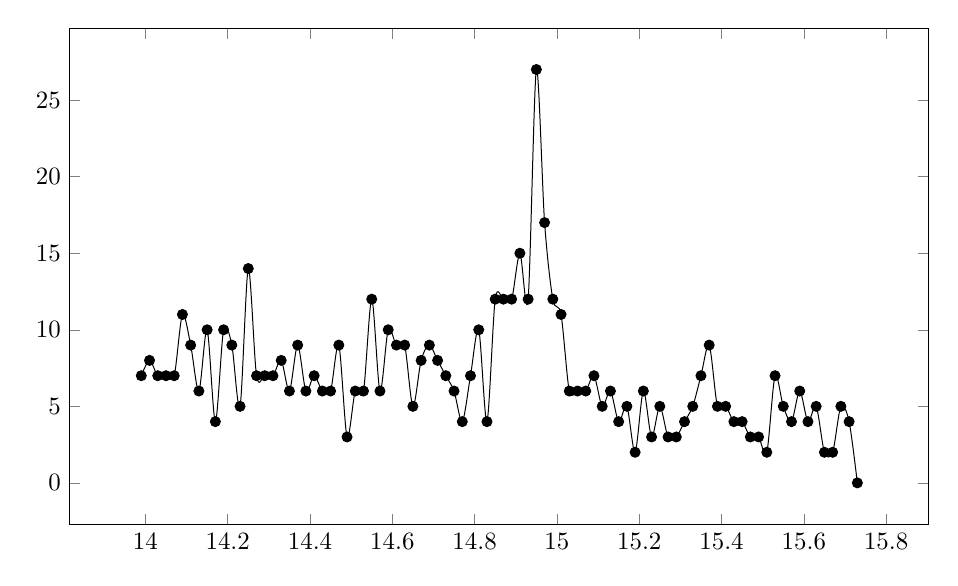
\begin{tikzpicture}[scale=0.9]
	\begin{axis}[
	scale only axis,
	%ymode=log, 
	width=\textwidth, 
	height=7cm
]
	\addplot [smooth,mark=*,black] table {%  plot X versus Y. This is original data.
	X		Y 

 13.990 7
 14.010 8
 14.030 7
 14.050 7
 14.070 7
 14.090 11
 14.110 9
 14.130 6
 14.150 10
 14.170 4
 14.190 10
 14.210 9
 14.230 5
 14.250 14
 14.270 7
 14.290 7
 14.310 7
 14.330 8
 14.350 6
 14.370 9
 14.390 6
 14.410 7
 14.430 6
 14.450 6
 14.470 9
 14.490 3
 14.510 6
 14.530 6
 14.550 12
 14.570 6
 14.590 10
 14.610 9
 14.630 9
 14.650 5
 14.670 8
 14.690 9
 14.710 8
 14.730 7
 14.750 6
 14.770 4
 14.790 7
 14.810 10
 14.830 4
 14.850 12
 14.870 12
 14.890 12
 14.910 15
 14.930 12
 14.950 27
 14.970 17
 14.990 12
 15.010 11
 15.030 6
 15.050 6
 15.070 6
 15.090 7
 15.110 5
 15.130 6
 15.150 4
 15.170 5
 15.190 2
 15.210 6
 15.230 3
 15.250 5
 15.270 3
 15.290 3
 15.310 4
 15.330 5
 15.350 7
 15.370 9
 15.390 5
 15.410 5
 15.430 4
 15.450 4
 15.470 3
 15.490 3
 15.510 2
 15.530 7
 15.550 5
 15.570 4
 15.590 6
 15.610 4
 15.630 5
 15.650 2
 15.670 2
 15.690 5
 15.710 4
 15.730 0
		}
	node[right,red] at (axis cs:38.460,992) {$2\Theta=38.460$}
	node[right,red] at (axis cs:44.700,441) {$2\Theta=44.700$}
	node[right,red] at (axis cs:65.020,1406) {$2\Theta=65.020$}
	node[above,red] at (axis cs:78.100,702) {$2\Theta=78.100$}	
	node[above,red] at (axis cs:85.10,41) {$2\Theta=82.340$};
	\end{axis}
	
\end{tikzpicture}





